%%%%%%%%%%%%%%%%%%%%%%%%%%%%%%%%%%%%%%%%%%%%%%%%%%%%%%%%%%%%%%%%%%%%%%%%%%%
%
%    phase1-AR.tex  (use only for Archival Research and Theory proposals; use phase1-GO.tex
%                     for General Observer and Snapshot proposals and phase1-DD.tex for GO/DD 
%                     proposals or use phase1-MC.tex for GO/MC rapid response proposals.
%                     
%
%    HUBBLE SPACE TELESCOPE
%    PHASE I ARCHIVAL & THEORETICAL RESEARCH PROPOSAL TEMPLATE 
%    FOR CYCLE 25 (2017)
%
%    Version 1.0, January 2017
%
%    Guidelines and assistance
%    =========================
%     Cycle 25 Announcement Web Page:
%
%         http://www.stsci.edu/hst/proposing/docs/cycle25announce 
%
%    Please contact the STScI Help Desk if you need assistance with any
%    aspect of proposing for and using HST. Either send e-mail to
%    help@stsci.edu, or call 1-800-544-8125; from outside the United
%    States, call [1] 410-338-1082.
%
%%%%%%%%%%%%%%%%%%%%%%%%%%%%%%%%%%%%%%%%%%%%%%%%%%%%%%%%%%%%%%%%%%%%%%%%%%%

% The template begins here. Please do not modify the font size from 12 point.

\documentclass[12pt,leqno]{article}


%%%%%%%%%%%%%%%%%%%%%%%%%%%%%%%%%%%%%%%%%%%%%%%%%%%%%%%%%%%%%
%  PREAMBLE: sets up compiler modes, loads packages, defines macros, etc
%  Steve Rodney, 2012
%%%%%%%%%%%%%%%%%%%%%%%%%%%%%%%%%%%%%%%%%%%%%%%%%%%%%%%%%%%%%


%%%%%%%%%%%%%%%%%%%%
% COMPILER MODES
%%%%%%%%%%%%%%%%%%%%

% Changetext mode : highlight modified text in bold blue font
\newif{\ifchangetext}
\changetextfalse

%% Read in the -options.tex file (generated by the Makefile)
%%  to set the compile-mode options
\InputIfFileExists{\jobname-options}


%%%%%%%%%%%%%%%%%%%%%%%%%%%%%%%
% changetext  mode settings
%%%%%%%%%%%%%%%%%%%%%%%%%%%%%%%
\ifchangetext
  % Changed text is highlighted in bold, blue font 
  \newcommand{\change}[1]{\textcolor{blue}{ \bf #1}}
  \newcommand{\changenote}[1]{\textcolor{blue}{ \bf #1}}
\else
  % Changed text is indistinguishable
  \newcommand{\change}[1]{#1}
  \newcommand{\changenote}[1]{}
\fi


%%%%%%%%%%%%%%%%%%%%
% PACKAGES INCLUDED
%%%%%%%%%%%%%%%%%%%%
%\usepackage{deluxetable}  % stand-alone version of AAStex's  deluxetable
\usepackage{longtable}
\usepackage{tabu}
\usepackage{booktabs}
\usepackage{array}
\usepackage{aas-macros}
\usepackage{phase1}
%\usepackage{journalnames} % Astro Journal abbreviations
\usepackage{natbib}   % reference citations and bibliography
\usepackage[svgnames]{xcolor}  % colored text (better than color)
\usepackage{graphicx}
\usepackage{amsmath}  % equations and such
%\usepackage{amssymb}  % extended symbols lib
\usepackage{setspace} % switch from double to single spacing
\usepackage{wrapfig}
\usepackage{float}
%\usepackage[linkcolor=blue,citecolor=darkgray,colorlinks=true]{hyperref}
%\usepackage{enumerate}% enumerated lists
%\usepackage{mathrsfs} % extended math fonts (mathscr)
%\usepackage{breqn}    % automatic line breaks for long equations
%\usepackage{multirow}  % muti-row table cells
%\usepackage{paralist} % inline enumeration (for Table ref lists)
%\usepackage{authblk}
%\usepackage{multicol}
\usepackage{sidecap} % captions beside figs
%\usepackage{subfig} % subfloats with independent captions
%\usepackage{subcaption} % subfloats with independent captions
%\usepackage[none]{hyphenat} % Suppress the hyphenating
%\usepackage{verbatim} % verbatim text formatting
%\usepackage{ulem} % for some underlining.
%\usepackage[usenames]{color}  % colored text
%\usepackage{colortbl}


\usepackage{multicol}

%\usepackage{etoolbox}
%\patchcmd{\thebibliography}{\section*{\refname}}
%    {\begin{multicols}{2}[\section*{\refname}]}{}{}
%\patchcmd{\endthebibliography}{\endlist}{\endlist\end{multicols}}{}{}

%%%%%%%%%%%%%%%%%%%%%%%%%%%%%%%%%%%%%%%%%%%%%%%%%%%
% PDF mode settings : Auto-select eps or pdf figures 
% based  on the compiler used (i.e. latex vs pdflatex)
%%%%%%%%%%%%%%%%%%%%%%%%%%%%%%%%%%%%%%%%%%%%%%%%%%%
%\DeclareGraphicsExtensions{.png,.pdf,.jpg}

%%%%%%%%%%%%%%%%%%%%%%%%%%%%%%%
% AUTHOR-DEFINED MACROS
%%%%%%%%%%%%%%%%%%%%%%%%%%%%%%%

% Time delay 
\def\dt{\ensuremath{\Delta t}}
\def\Dl{\ensuremath{D_L}}
\def\Ds{\ensuremath{D_S}}
\def\Dls{\ensuremath{D_{LS}}}

% dagger for marking primary targets
\def\dag{\ensuremath{^{\dagger}}}

% plus-minus symbols for statistical or systematic errors
\def\pmstat{\ensuremath{\substack{\pm \\ \mbox{\scalebox{0.45}{stat}}}}}
\def\pmsys{\ensuremath{\substack{\pm \\ \mbox{\scalebox{0.45}{sys}}}}}


% prompt Ia fraction
\def\fp{\ensuremath{f_{P}}}
\def\fP{\ensuremath{f_{P}}}

% STARDUST probabilities
\def\pIa{\ensuremath{p_{Ia}}}
\def\pIaz{\ensuremath{p_{Ia,z}}}
\def\pIahost{\ensuremath{p_{Ia,host}}}

% General purpose usefulness:
\newcommand{\etal}{{et al.~}}                                             
\def\eg{{e.g.}}
\def\ie{{i.e.}}
\def\etc{{etc.}}
\newcommand{\lta}{\lesssim}                                               
\newcommand{\gta}{\gtrsim}                                                
\newcommand{\gt}{\gtsim}

% Cosmology:
\def\Om{\ensuremath{\Omega_{\rm m}}}
\def\Ot{\ensuremath{\Omega_{\rm tot}}}
\def\Ob{\ensuremath{\Omega_{\rm b}}}
\def\OL{\ensuremath{\Omega_{\Lambda}}}
\def\Ok{\ensuremath{\Omega_{\rm k}}}
\def\om{\ensuremath{\omega_{\rm m}}}
\def\ob{\ensuremath{\omega_{\rm b}}}
\def\wo{\ensuremath{w_0}}
\def\wa{\ensuremath{w_{\rm a}}}
\def\lcdm{$\Lambda$CDM}
\def\LCDM{$\Lambda$CDM}
\def\wcdm{$w$CDM}
\def\Ho{\ensuremath{H_0}}
\def\DA{\ensuremath{D_A}}
\def\DL{\ensuremath{D_L}}

% Astronomy:
\def\arcsec{\ensuremath{^{\prime\prime}}} 
\def\kms{\ensuremath{{\rm km s}^{-1}}}
\def\hgpcq{\mbox{$h^{-3}$Gpc$^3$}}
\def\hmpcq{\mbox{$h^{-3}$Mpc$^3$}}
\def\perhmpcq{\mbox{$h^{3}$Mpc$^{-3}$}}
\def\hmpc{\mbox{$h^{-1}$Mpc}}
\def\hmpci{\mbox{$h$\,Mpc$^{-1}$}}
\def\mpc{\mbox{Mpc}}
\def\mpci{\mbox{Mpc$^{-1}$}}
\def\mpcq{\mbox{Mpc$^{-3}$}}
\def\Msun{\mbox{M$_{\odot}$}}
\def\Av{\mbox{$A_V$}}
\def\Rv{\mbox{$R_V$}}

% Supernovae : 
\newcommand{\SNuVol}{\ensuremath{10^{-4}~\mbox{yr}^{-1}~\mbox{Mpc}^{-3}~{\mbox{h}_{70}}^{3}}}
\newcommand{\CCSN}{CC\,SN}
\newcommand{\CCSNe}{CC\,SN}
\newcommand{\TNSN}{TN\,SN}
\newcommand{\TNSNe}{TN\,SNe}
\newcommand{\SNIa}{SN\,Ia}
\newcommand{\SNeIa}{SN\,Ia}
\newcommand{\SNRz}{SNR($z$)}
\def\Mch{\mbox{M$_{\rm Ch}$}}
\def\Ni{\ensuremath{^{56}\mbox{Ni}}}
\newcommand{\dmfifteen}{\ensuremath{\Delta\mbox{m}_{15}}}
\newcommand{\deltamfifteen}{\ensuremath{\Delta\mbox{m}_{15}}}
\newcommand{\NM}{\ensuremath{\mbox{\rm N}_{Ia}/\mbox{M}_{*}}}

\def\galsnid{{\it galsnid}}

% SNANA / SALT2
\def\xone{\ensuremath{x_{1}}}
\def\C{\ensuremath{\mathcal{C}}}


% Missions:
\def\HST{{\it HST}}
\def\Hubble{{\it Hubble}}
\def\Hubbles{{\it Hubble's}}
\def\Spitzer{{\it Spitzer}}
\def\Chandra{{\it Chandra}}
\def\Herschel{{\it Herschel}}
\def\XMM{{\it XMM}}


%%%%%%%%%%%%%%%%%%%%%%%%%%%%%%%
% Page Setup 
%%%%%%%%%%%%%%%%%%%%%%%%%%%%%%%
\renewcommand{\topfraction}{0.9}
\renewcommand{\bottomfraction}{0.9}
\renewcommand{\textfraction}{0.1}
\renewcommand{\floatpagefraction}{0.9}
\renewcommand{\dbltopfraction}{0.9}
\renewcommand{\dblfloatpagefraction}{0.9}



%%%%%%%%%%%%%%%%%%%%%%%%%%%%%%%%%%%%
%% Figure placement shortcuts    
%%%%%%%%%%%%%%%%%%%%%%%%%%%%%%%%%%%%


\newcommand{\insertfigwide}[2] {
\begin{figure*}
\begin{center}
\resizebox{\textwidth}{!}{\includegraphics{{#1}}}
\caption{{#2}}
\end{center}
\end{figure*}
}

\newcommand{\insertfigdouble}[3] {
\begin{figure*}
\begin{center}
\resizebox{0.45\textwidth}{!}{\includegraphics{{#1}}}
\resizebox{0.45\textwidth}{!}{\includegraphics{{#2}}}
\caption{{#3}}
\end{center}
\end{figure*}
}

\newcommand{\insertfigquad}[5] {
\begin{figure*}
\begin{center}
\resizebox{0.48\textwidth}{!}{\includegraphics{{#1}}}
\resizebox{0.48\textwidth}{!}{\includegraphics{{#2}}}
\resizebox{0.48\textwidth}{!}{\includegraphics{{#3}}}
\resizebox{0.48\textwidth}{!}{\includegraphics{{#4}}}
\caption{{#5}}
\end{center}
\end{figure*}
}

\newcommand{\insertfig}[2] {
\begin{figure}
\begin{center}
\resizebox{\columnwidth}{!}{\includegraphics{{#1}}}
\caption{{#2}}
\end{center}
\end{figure}
}
\begin{document}

%   1. SCIENTIFIC JUSTIFICATION
%       (see Section 9.1 of the Call for Proposals)
%
%

\justification          % Do not delete this command.

\begin{figure}[b]
\centering
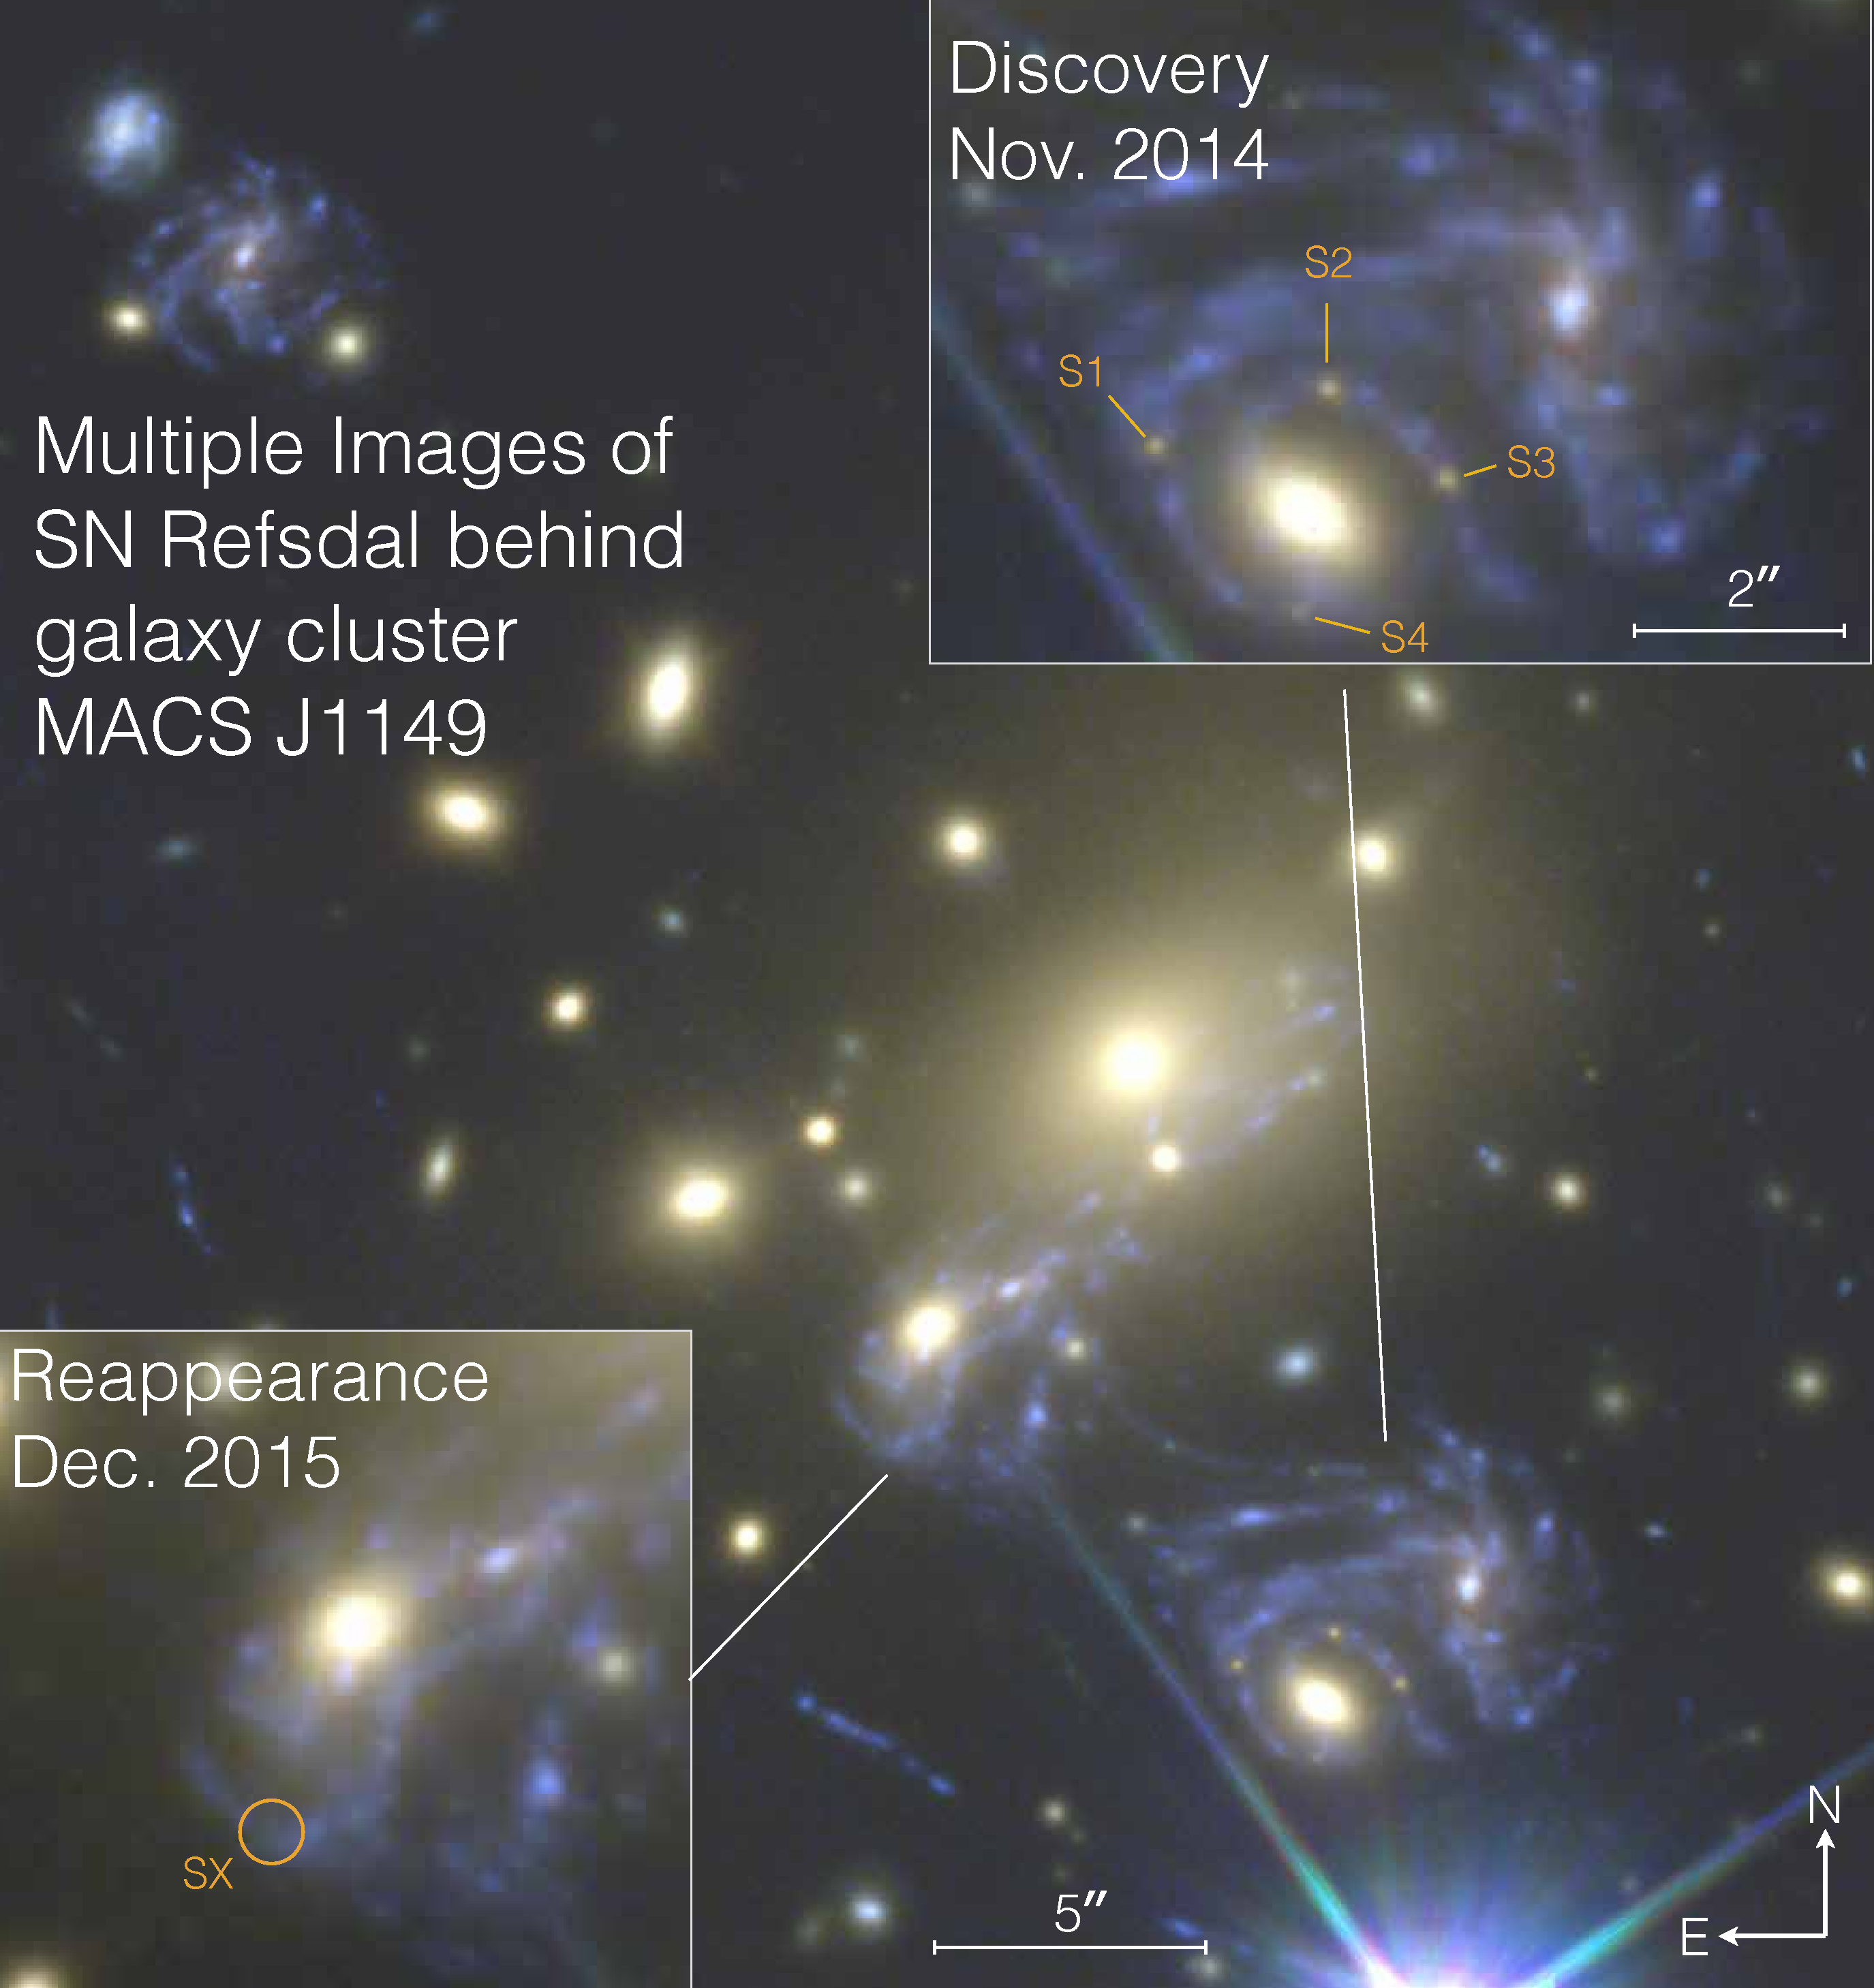
\includegraphics[height=3.6in]{FIG/refsdal_summary2}
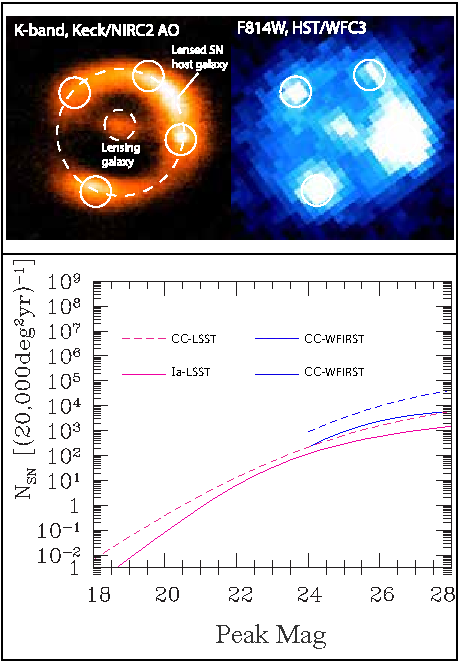
\includegraphics[height=3.6in]{FIG/lensed3}
\caption{
(A) MACS J1149.6+2223 field, showing the positions of the three primary
images of the SN Refsdal host galaxy. SN
Refsdal appears as four point sources in an Einstein Cross
configuration in the southeast spiral arm of image 1.1. (B) HST/WFC3 observation
of iPTF16geu, revealing four point sources and (C) NIR Keck observation, with the 
Einstein ring of the host galaxy clearly visible, adapted from \citet{Goobar:2016}. (D)
Expected numbers of Type Ia and Core Collapse SNe for LSST $(i_{peak,lim})$ and 
WFIRST $(H_{peak,lim})$, adapted from \citet{Oguri:2010a}.}
\end{figure}%

\forceindent The seminal work of \citet{Refsdal:1964} first showed how a
gravitationally lensed supernova (SN) resolved into multiple images
could be used as a cosmological tool.  Now, some 50 years later, HST
is playing an integral role in the long-awaited first observations of
such events (Figure 1).  HST observations caught the first
multiply-imaged SN, called ``SN Refsdal"---a core-collapse SN lensed
by both a galaxy cluster and a single galaxy (Kelly et al. 2015). This
was followed by the first multiply-imaged Type Ia SN (iPTF16geu),
resolved with HST imaging \citep{Goobar:2016}.  As the light for each
of the multiple images follows a different path through the expanding
universe and through the lensing potential, the SN images appear
delayed by hours (for galaxy-scale lenses) or years (for cluster-scale
lenses). For objects like SN Refsdal, measurement of this time delay
can be used as a precise test of cluster lens
models \citep{Treu:2015b}. For a SN like iPTF16geu, the time delay can
lead to a direct constraint on the Hubble constant that is completely
independent of the local distance ladder.

Preliminary time delay
measurements have been made, but for both SNe these are limited by the
need to include complex microlensing effects \citep{Rodney:2016,
More:2016}.  {\bf We propose to re-analyze the HST observations for
these two lensed SNe, improving the photometry and including the
significant yet previously ignored effects of microlensing.  We will
develop an open-source software package in the course of this work,
optimized for multiply-imaged SNe, that will enable precise time delay
measurements to be made for hundreds of lensed SNe expected in the
LSST/WFIRST era.}

To improve the control of systematic biases in the SN photometry, our
reanalysis will use both the \textit{PythonPhot} and
the \textit{DOLPHOT} packages. We will also measure the photometry in
single-exposure images to identify any deviations at very short
timescales, indicative of very rapid microlensing
events. \cite{Rodney:2016} measured the SN Refsdal photometry using a
static point-spread function (PSF) derived from standard
stars. However, as we know that the HST PSF does undergo subtle
variations due to telescope ``breathing," our re-analysis will use
foreground stars within the MACS1149 imaging datasets to define a
variable PSF model \textbf{The improved photometric accuracy and
precision will be critical for identifying and correcting subtle
microlensing effects.}

Microlensing refers to small-scale gravitational lensing perturbations
due to massive objects along the light path of any one image of a
multiply-imaged SN. This causes distortions in the SN light curves
that limit the precision that can be achieved in
their time delay measurements \citep{Dobler:2006}. Despite noting this significant
source of uncertainty, early analyses of SN Refsdal and iPTF16geu have
ignored microlensing due to its
complexity \citep{More:2016,Rodney:2016}. In preparing this proposal,
we have already used flexible functions to get a preliminary
measurement of microlensing for SN Refsdal (Figure 2), and it is
\textbf{clear that microlensing must be taken into account.} 
Therefore, we will analyze the effects of microlensing on a
multiply-imaged SN for the and ensure they can be accurately accounted
for in future SN analysis.

\textbf{The next decade is expected to yield observations
of tens to hundreds of multiply-imaged SNe} \citep{Oguri:2010},
yet \textbf{there is no public software package for analyzing
multiply-imaged SNe.}  A core product of this work will be an
open-source Python package for use in this and future SN
analyses. This new will be used to deliver new time delay measurements 
for SN Refsdal make , providing an important
independent check of such a measurement for the first time.

The discovery of SN iPTF16geu suggests that the \textbf{rate of
strongly lensed Type Ia SNe is likely much higher than previously
thought}, with implications for our constraints on $H_0$, the study of
galaxy sub-structures, and tests of theories of modified gravity
\citep{Goobar:2016,More:2016}. If the number of lensed Type
Ia SNe observed in the LSST/WFIRST era follows these predictions, then
it will be essential to have a publicly available, standardized tool
in place for accurate time delay and magnification
measurements. Reanalysis of these two lensed SNe offers a unique
chance to develop the tools necessary for analyzing many new lensed
SNe in the coming years, finally realizing the 50-year promise of
using lensed SNe as a new cosmological probe.

\begin{figure}[p]
\centering
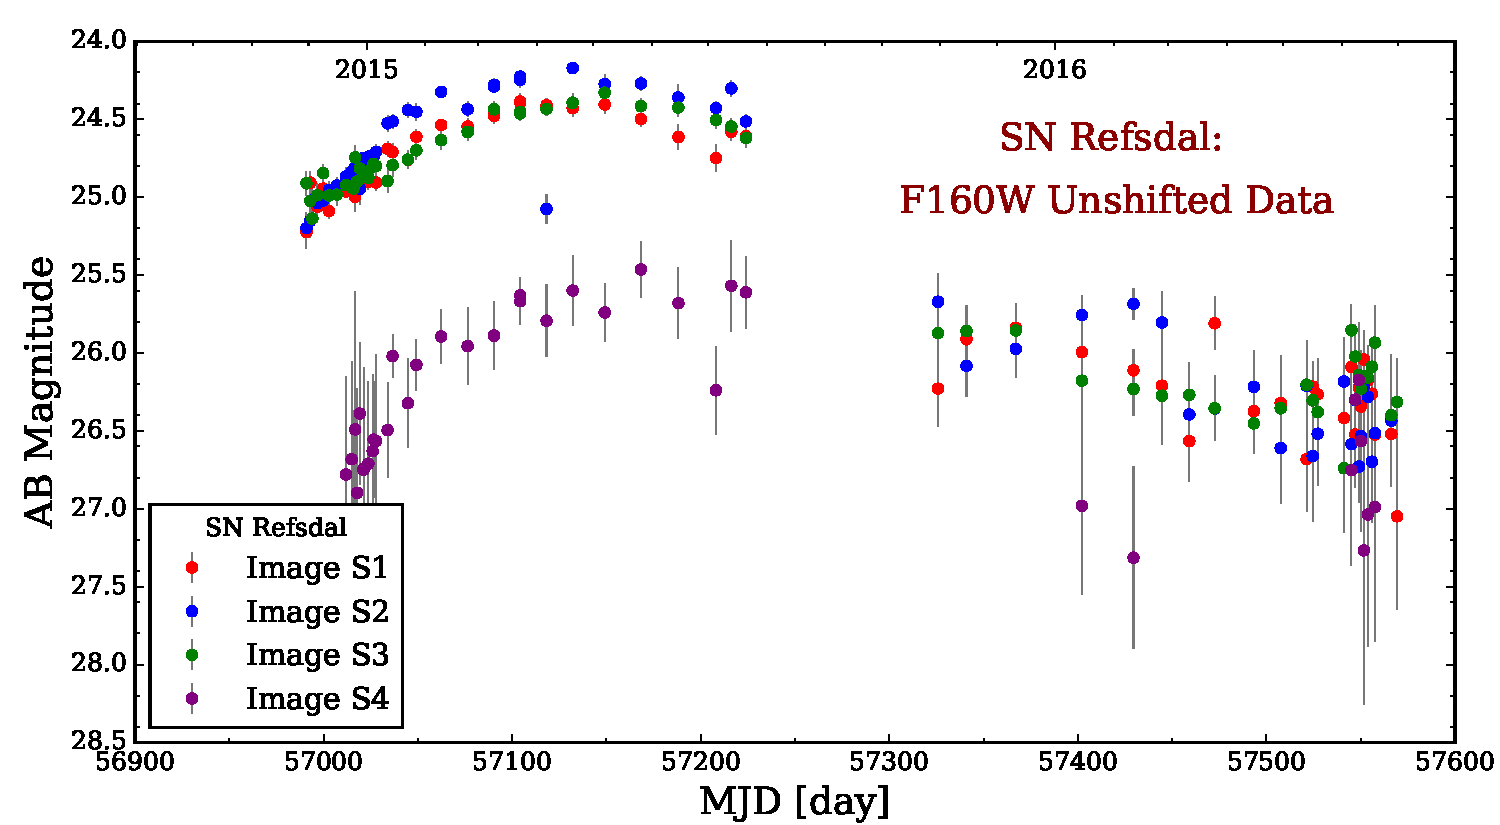
\includegraphics[width=.7\textwidth]{FIG/points_plot_2017.pdf}
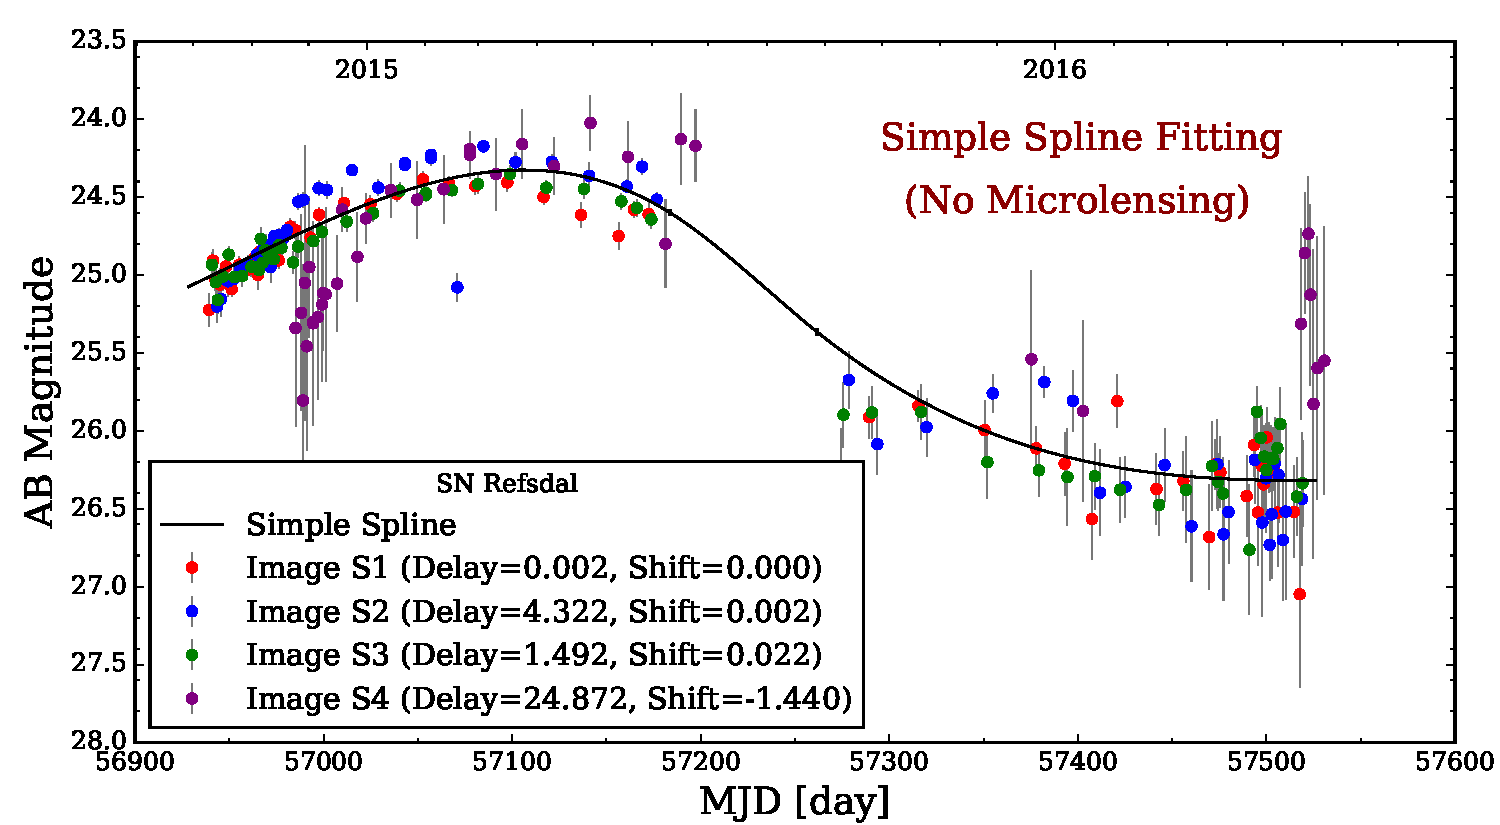
\includegraphics[width=.7\textwidth]{FIG/refs_plot_2017.pdf}
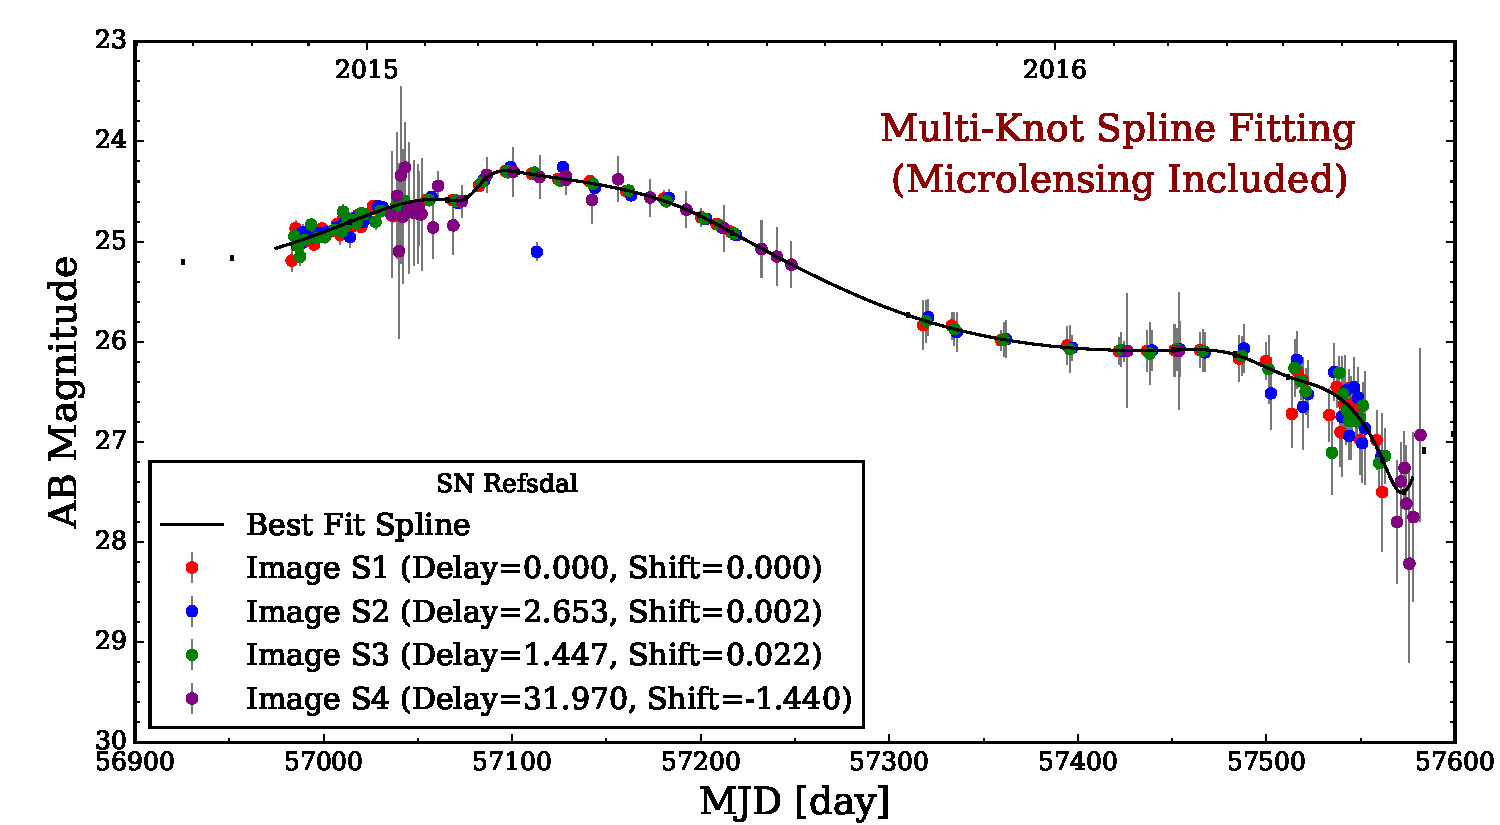
\includegraphics[width=.7\textwidth]{FIG/spline_plot_2017.pdf}
\caption{(Top) HST F160W data representing the four images of SN
Refsdal (Figure 1A), with no lensing or time shifts. (Middle) Method of
fitting the SN Refsdal light curves from Rodney et al. 2016, which did
not consider microlensing effects. (Bottom) Preliminary results from 
this work using a multi-knot spline to fit the data. This method 
includes microlensing effects, which leads to a slight adjustment in 
time delay measurements. }
\end{figure}

\bigskip



\
%%%%%%%%%%%%%%%%%%%%%%%%%%%%%%%%%%%%%%%%%%%%%%%%%%%%%%%%%%%%%%%%%%%%%%%%%%%
%   2. ANALYSIS PLAN
%       (see Section 9.6 of the Call for Proposals)
%
%
\describearchival       % Do not delete this command.
\forceindent There are 64 relevant datasets in the HST archive that will be used in this work: 58 
intersecting the coordinates of MACSJ1149, and 8 intersecting the coordinates of SN iPTF16geu. 
The data intersecting MACSJ1149 are from the WFC3-IR and 
ACS-WFC instruments, and span April 22, 2004-October 30, 2016 with HST Project IDs: 9722,\ 
10493,\ 12068,\ 12197,\ 13504,\ 13459,\ 14041,\  13790,\ 14199, and 14208. The data intersecting 
SN iPTF16geu are from the WFC3-IR instrument, and span October 20-November 17, 2016 with HST
Project ID 14862.

The required HST datasets amount to a relatively small volume of data.
All datasets will be requested from the archive at once, at the start
of the project. We will start with the FLT files, and will process
them through a modified version of the HST data processing pipeline
that was originally developed for the CANDELS and CLASH SN surveys
\citep{Rodney:2014}.  This pipeline uses a custom processing sequence
with AstroDrizzle and TweakReg to segregate the data into epochs,
combine each epoch of HST imaging exposures, register them to a common
co ordinate system, and generate difference images suitable for SN
detection and photometric measurements. This pipeline was updated for
use in SN searches related to the Frontier Fields, and is now publicly
available (\url{https://github.com/srodney/sndrizpipe}). 

This pipeline will be revised and improved again for this work, adding
additional steps to remove persistence artifacts that might impact the
photometry of the SN targets and/or the foreground stars that will be
used to define a time-varying PSF model. For the initial measurement
of the time delays of SN Refsdal, special data processing steps were
required to address contamination of the SN by diffraction spikes from
a 15th-magnitude star in the foreground \citep{Rodney:2016}.  Revision
and improvement of this contamination removal will be a critical step
for increasing the precision of the photometry for SN Refsdal.



%\begin{tabular}{ccccc}
%\centering
%Start Date & Start MJD &Total Integration Time (s)&Instrument & HST Program ID\\
%\hline
%\hline
%2004 Apr 22.6&53117.6&63630&ACS&9722\\
%2006 May 25.5&53880.5&15288&ACS&10493\\
%2010 Dec 04.9&55534.9&14462&ACS&12068\\
%2010 Dec 05.0&55535.0&10058.7&WFC3&12068\\
%2011 Jan 16.0&55577.0&14532&ACS&12068\\
%2011 Jan 16.0&55577.0&10058.7&WFC3&12068\\
%2011 Jan 30.6&55591.6&14462&ACS&12068\\
%2011 Jan 30.7&55591.7&10058.7&WFC3&12068\\
%2011 Feb 13.3&55605.3&14329&ACS&12068\\
%2011 Feb 13.3&55605.3&64691&WFC3&12068\\
%2011 Feb 27.0&55619.0&14182&ACS&12068\\
%2011 Feb 27.1&55619.1&9758.7&WFC3&12068\\
%2011 Feb 27.5&55619.5&13916&ACS&12068\\
%2011 Feb 27.6&55619.6&28386.8&WFC3&12068\\
%2011 Mar 09.8&55629.8&14595&ACS&12068\\
%2011 Mar 09.8&55629.8&10058.67676&WFC3&12068\\
%2012 Feb 07.9&55964.9&22387.7&WFC3&12197\\
%2013 Nov 02.2&56598.2&20632.9&WFC3&13504\\
%2013 Nov 12.8&56608.8&309120&WFC3&13389\\
%2014 Feb 23.4&56711.4&71728.7&WFC3&13459\\
%2014 Apr 14.7&56761.7&36722&ACS&13504\\
%2014 Nov 03.1&56964.1&51234.8&WFC3&13459\\
%2014 Nov 11.0&56972.0&20693.9&WFC3&13459\\
%2014 Nov 20.0&56981.0&20847&WFC3&13504\\
%2014 Nov 20.8&56981.8&190423&WFC3&13504\\
%2014 Nov 24.1&56985.1&65170&WFC3&14041\\
%2014 Nov 29.9&56990.9&55623&WFC3&13790\\
%2014 Dec 11.8&57002.8&154329&WFC3&13504\\
%2014 Dec 22.9&57013.9&74312&WFC3&13790\\
%2014 Dec 23.7&57014.7&10232&WFC3&14041\\
%2014 Dec 23.8&57014.8&88988&WFC3&13504\\
%2014 Dec 25.6&57016.6&51161&WFC3&14041\\
%2014 Dec 26.7&57017.7&44494&WFC3&13504\\
%2014 Dec 27.6&57018.6&92091&WFC3&14041\\
%2014 Dec 29.5&57020.5&44494&WFC3&13504\\
%2014 Dec 29.7&57020.7&71626&WFC3&14041\\
%2015 Jan 01.7&57023.7&44494&WFC3&13504\\
%2015 Jan 02.7&57024.7&20465&WFC3&14041\\
%2015 Jan 03.4&57025.4&44494&WFC3&13504\\
%2015 Jan 03.7&57025.7&40929&WFC3&14041\\
%2015 Jan 04.4&57026.4&44494&WFC3&13504\\
%2015 Jan 04.8&57026.8&20465&WFC3&14041\\
%2015 Jan 05.7&57027.7&65341&WFC3&13504\\
%2015 Jan 11.9&57033.9&86234&WFC3&13790\\
%2015 Apr 19.4&57131.4&68068&ACS&13504\\
%2015 Apr 20.1&57132.1&9106&WFC3&13790\\
%2015 Apr 20.5&57132.5&748076&ACS&13504\\
%2015 May 07.0&57149.0&9106&WFC3&13790\\
%2015 May 07.4&57149.4&314090&ACS&13504\\
%2015 May 26.3&57168.3&57999&WFC3&13790\\
%2015 Oct 30.8&57325.8&144163&WFC3&14199\\
%2016 May 16.3&57524.3&32850&WFC3&14208\\
%2016 May 16.5&57524.5&28964&WFC3&14199\\
%2016 May 23.3&57531.3&9896&WFC3&14208\\
%2016 May 23.4&57531.4&14604&ACS&14208\\
%2016 May 24.0&57532.0&183128&WFC3&14199\\
%2016 Oct 30.2&57691.2&&9670&WFC3&14199\\
%\end{tabular} 
%WFC=43, ACS=14



% Enter your analysis plan here.

%%%%%%%%%%%%%%%%%%%%%%%%%%%%%%%%%%%%%%%%%%%%%%%%%%%%%%%%%%%%%%%%%%%%%%%%%%%

%   3. MANAGEMENT PLAN
%       (see Section 9.7 of the Call for Proposals)
%
%  Provide a concise, but complete, management plan. This plan will be used
%  by the review panels to assess the likely scale of the proposed research
%  program. Proposers should include a schedule of the work required to
%  achieve the scientific goals of the program, a description of the roles of the
%  PI, CoIs, postdocs, and students who will perform the work, and a plan to
%  disseminate the results to the community.
%
\budgetnarrative       % Do not delete this command. CALLS the Management Plan header in the Style File (IGNORE the command name of budgetnarrative
\forceindent The first stage of this project is to produce an open-source software
package called Supernova Time Delays ({\tt SNTD}). The software is being
developed as an open-source project, and is already publicly
accessible on github (\url{https://github.com/jpierel14/sntd}).  {\tt SNTD}
relies on two other public software packages: Python Curve Shifting
({\tt PyCS}; \citealt{Tewes:2013a}) a tool developed for measurement of
quasar time delays, and the SN light curve analysis package {\tt sncosmo}
(\citep{Barbary:2014}). Our further development of {\tt SNTD} will proceed in three steps: 1)
Integrate SNCosmo and PyCS, producing a tool that can model
SN light curve data with the abilities present in either software
package; 2) Extend and optimize the lensing and microlensing algorithm
present in PyCS for SNe; 3) Simulate a large number of multiply-imaged
SN light curves using SNCosmo and test the ability of SNTD to
simultaneously determine SN and lensing parameters. This work will be
done primarily by graduate student PI Roberts-Pierel, under the
guidance of Co-I Rodney at USC.  We anticipate this will require 4-6
months of full time effort from the PI.

In parallel with the software development, we will improve the
photometry of the two multiply-imaged SNe (Refsdal and iPTF16geu) by
1) reprocessing the HST images using the most up-to-date AstroDrizzle
software; 2) developing new time-variable PSF models, based on stellar
sources within each image; and 3) deriving new photometric time
series, using multiple photometry packages to extract photometry from
both the template-subtracted difference images and directly from the
FLT files. Although SN Refsdal appeared in the Hubble Frontier Fields,
for this work it is necessary to reprocess the data separately from
the official HFF products, because we need to break it up into
separate epochs.  This component will require 4-6 months of part-time
work from the two Co-I's, supplemented by additional effort from the
grad student PI.

For the conclusion of this project, we will use the new SNTD package
to measure improved gravitational lensing parameters for SN Refsdal
and iPTF16geu.   We anticipate that the
SNTD package and the results of the new lensing analyses will be
separately published within 12 months of the start of this project.

\bibliographystyle{apjbrief}

\bibliography{bibs/bibdesk}

\end{document}          % End of proposal. Do not delete this line.
                        % Everything after this command is ignored.

